%%%%%%%%%%%%%%%%%%%%%%%%%%%%%%%%%%%%%%%%%%%%%%%%%%%%%%%%%%%%%%%%%%%%%%%%%%%%%%%%
%Tutorial slides on Python.
%
% Author: FOSSEE
% Copyright (c) 2009-2016, FOSSEE, IIT Bombay
%%%%%%%%%%%%%%%%%%%%%%%%%%%%%%%%%%%%%%%%%%%%%%%%%%%%%%%%%%%%%%%%%%%%%%%%%%%%%%%%

\documentclass[14pt,compress]{beamer}

% Modified from: generic-ornate-15min-45min.de.tex
\mode<presentation>
{
  \usetheme{Warsaw}
  \useoutertheme{infolines}
  \setbeamercovered{transparent}
}

% Remove navigation symbols.
\setbeamertemplate{navigation symbols}{}

\usepackage[english]{babel}
\usepackage[latin1]{inputenc}
%\usepackage{times}
\usepackage[T1]{fontenc}

% Taken from Fernando's slides.
\usepackage{ae,aecompl}
\usepackage{mathpazo,courier,euler}
\usepackage[scaled=.95]{helvet}

\definecolor{darkgreen}{rgb}{0,0.5,0}

\usepackage{listings}
\lstset{language=Python,
    basicstyle=\ttfamily\bfseries,
    commentstyle=\color{red}\itshape,
  stringstyle=\color{darkgreen},
  showstringspaces=false,
  keywordstyle=\color{blue}\bfseries}

%%%%%%%%%%%%%%%%%%%%%%%%%%%%%%%%%%%%%%%%%%%%%%%%%%%%%%%%%%%%%%%%%%%%%%
% Macros
\setbeamercolor{emphbar}{bg=blue!20, fg=black}
\newcommand{\emphbar}[1]
{\begin{beamercolorbox}[rounded=true]{emphbar}
      {#1}
 \end{beamercolorbox}
}
\newcounter{time}
\setcounter{time}{0}
\newcommand{\inctime}[1]{\addtocounter{time}{#1}{\tiny \thetime\ m}}

\newcommand{\typ}[1]{\lstinline{#1}}

\newcommand{\kwrd}[1]{ \texttt{\textbf{\color{blue}{#1}}}  }

\newcommand\BackgroundPicture[1]{%
  \setbeamertemplate{background}{%
      \parbox[c][\paperheight]{\paperwidth}{%
      \vfill \hfill
        \pgfimage[width=1.0\paperwidth,height=1.0\paperheight]{#1}
 \hfill \vfill
}}}

% For non-wide pictures, set the width so that the height scales
% appropriately.
\newcommand\BackgroundPictureWidth[1]{%
  \setbeamertemplate{background}{%
      \parbox[c][\paperheight]{\paperwidth}{%
      \vfill \hfill
        \pgfimage[width=1.0\paperwidth]{#1}
 \hfill \vfill
}}}

% For shorter pictures, set the height so that the width scales
% appropriately.
\newcommand\BackgroundPictureHeight[1]{%
  \setbeamertemplate{background}{%
      \parbox[c][\paperheight]{\paperwidth}{%
      \vfill \hfill
        \pgfimage[height=1.0\paperheight]{#1}
 \hfill \vfill
}}}

%%%%%%%%%%%%%%%%%%%%%%%%%%%%%%%%%%%%%%%%%%%%%%%%%%%%%%%%%%%%%%%%%%%%%%
% Title page
\title[Introduction]{Introductory Scientific Computing with
Python}
\subtitle{Introduction to Python}

\author[FOSSEE] {FOSSEE}

\institute[IIT Bombay] {Department of Aerospace Engineering\\IIT Bombay}
\date[] {Mumbai, India
}
%%%%%%%%%%%%%%%%%%%%%%%%%%%%%%%%%%%%%%%%%%%%%%%%%%%%%%%%%%%%%%%%%%%%%%

%\pgfdeclareimage[height=0.75cm]{iitmlogo}{iitmlogo}
%\logo{\pgfuseimage{iitmlogo}}


%% Delete this, if you do not want the table of contents to pop up at
%% the beginning of each subsection:
\AtBeginSubsection[]
{
  \begin{frame}<beamer>
    \frametitle{Outline}
    \tableofcontents[currentsection,currentsubsection]
  \end{frame}
}

\AtBeginSection[]
{
  \begin{frame}<beamer>
    \frametitle{Outline}
    \tableofcontents[currentsection,currentsubsection]
  \end{frame}
}

% If you wish to uncover everything in a step-wise fashion, uncomment
% the following command:
%\beamerdefaultoverlayspecification{<+->}

%%\includeonlyframes{current,current1,current2,current3,current4,current5,current6}

%%%%%%%%%%%%%%%%%%%%%%%%%%%%%%%%%%%%%%%%%%%%%%%%%%%%%%%%%%%%%%%%%%%%%%
% DOCUMENT STARTS
\begin{document}

\begin{frame}
  \maketitle
\end{frame}

\begin{frame}
  \frametitle{Acknowledgement}
  \Large
  \begin{center}
    \alert{FOSSEE group (\url{fossee.in})} \\
    based at\\
    \alert{IIT Bombay}\\
    and funded by\\
    The National Mission on Education through ICT, \\
    \alert{Ministry of HRD, India}
  \end{center}
\end{frame}


\begin{frame}[plain]
    \begin{center}
        \Huge
        Why Python?
        \vspace*{1in}

        For Scientific Computing?
    \end{center}

\end{frame}

\begin{frame}
  \frametitle{Need: Toolkit for diversity}
  \Large
     \begin{itemize}
        \item Numeric and Symbolic
        \item Exploration and Visualization
        \item High performance
        \item Parallel computing
        \item User interfaces, Web
        \item Other tasks
  \end{itemize}
\end{frame}

\begin{frame}[plain]
  \frametitle{Why Python?}
  \Large
  \begin{itemize}
  \item Easy to read and learn
  \item Powerful interactive interpreter
  \item Scalable, general purpose
  \item High-level, modular
  \item Procedural, OO, functional
  \end{itemize}
\end{frame}

\begin{frame}[plain]
  \frametitle{Why Python?}
  \Large
  \begin{itemize}
  \item Extensive libraries
  \item Rapid application development
  \item Interface to C++, C and FORTRAN
  \item Cross-platform
  \item Open Source
  \end{itemize}
\end{frame}


\begin{frame}[plain]
  \frametitle{Requirements: numeric computation}

    \begin{center}
    \pgfimage[height=3.5in]{data/intro/scipy_screenie}

    \end{center}

\end{frame}

\begin{frame}[plain]
  \frametitle{SciPy}
  \begin{itemize}
  \item Linear algebra
  \item Numerical integration
  \item Fourier transforms
  \item Signal processing
  \item Special functions
  \item Statistics
  \item Optimization
  \item Image processing
  \item ODE solvers
    \vspace*{0.2in}
  \item Uses LAPACK, QUADPACK, ODEPACK, FFTPACK etc. from netlib
  \end{itemize}
\end{frame}

\begin{frame}[plain]
    \frametitle{Requirement: Exploration/Visualization}
    \begin{center}
    \pgfimage[height=3.0in]{data/intro/mayavi-ipython}
    \end{center}
  \end{frame}

\begin{frame}[plain]
  \frametitle{3D visualization with Mayavi2}
      \vspace*{-0.3in}
  \begin{center}
    \hspace*{-0.3in}\pgfimage[width=4.75in]{data/intro/m2_app}
  \end{center}
\end{frame}

\begin{frame}[plain]
    \frametitle{Requirement: HPC, parallel computing}
    \begin{center}
    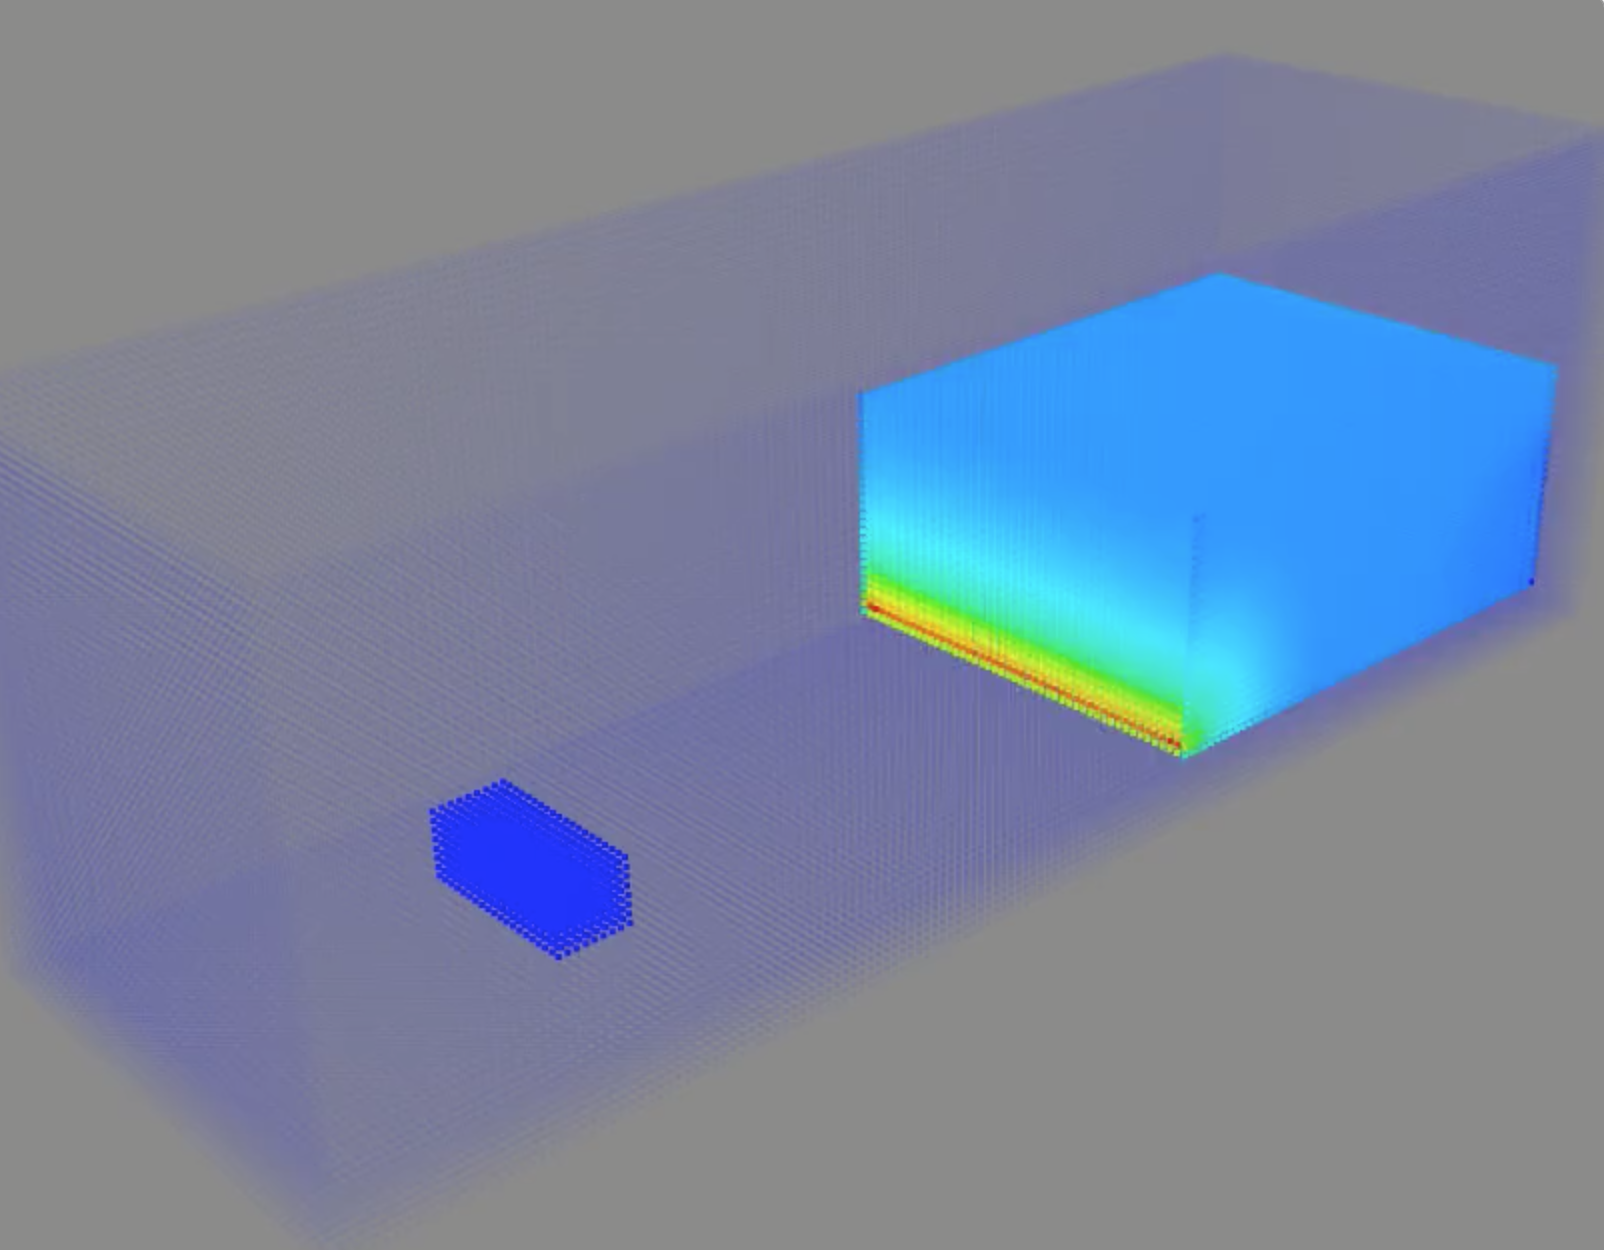
\includegraphics[height=1.75in]{data/intro/dam_break_poster_0}
    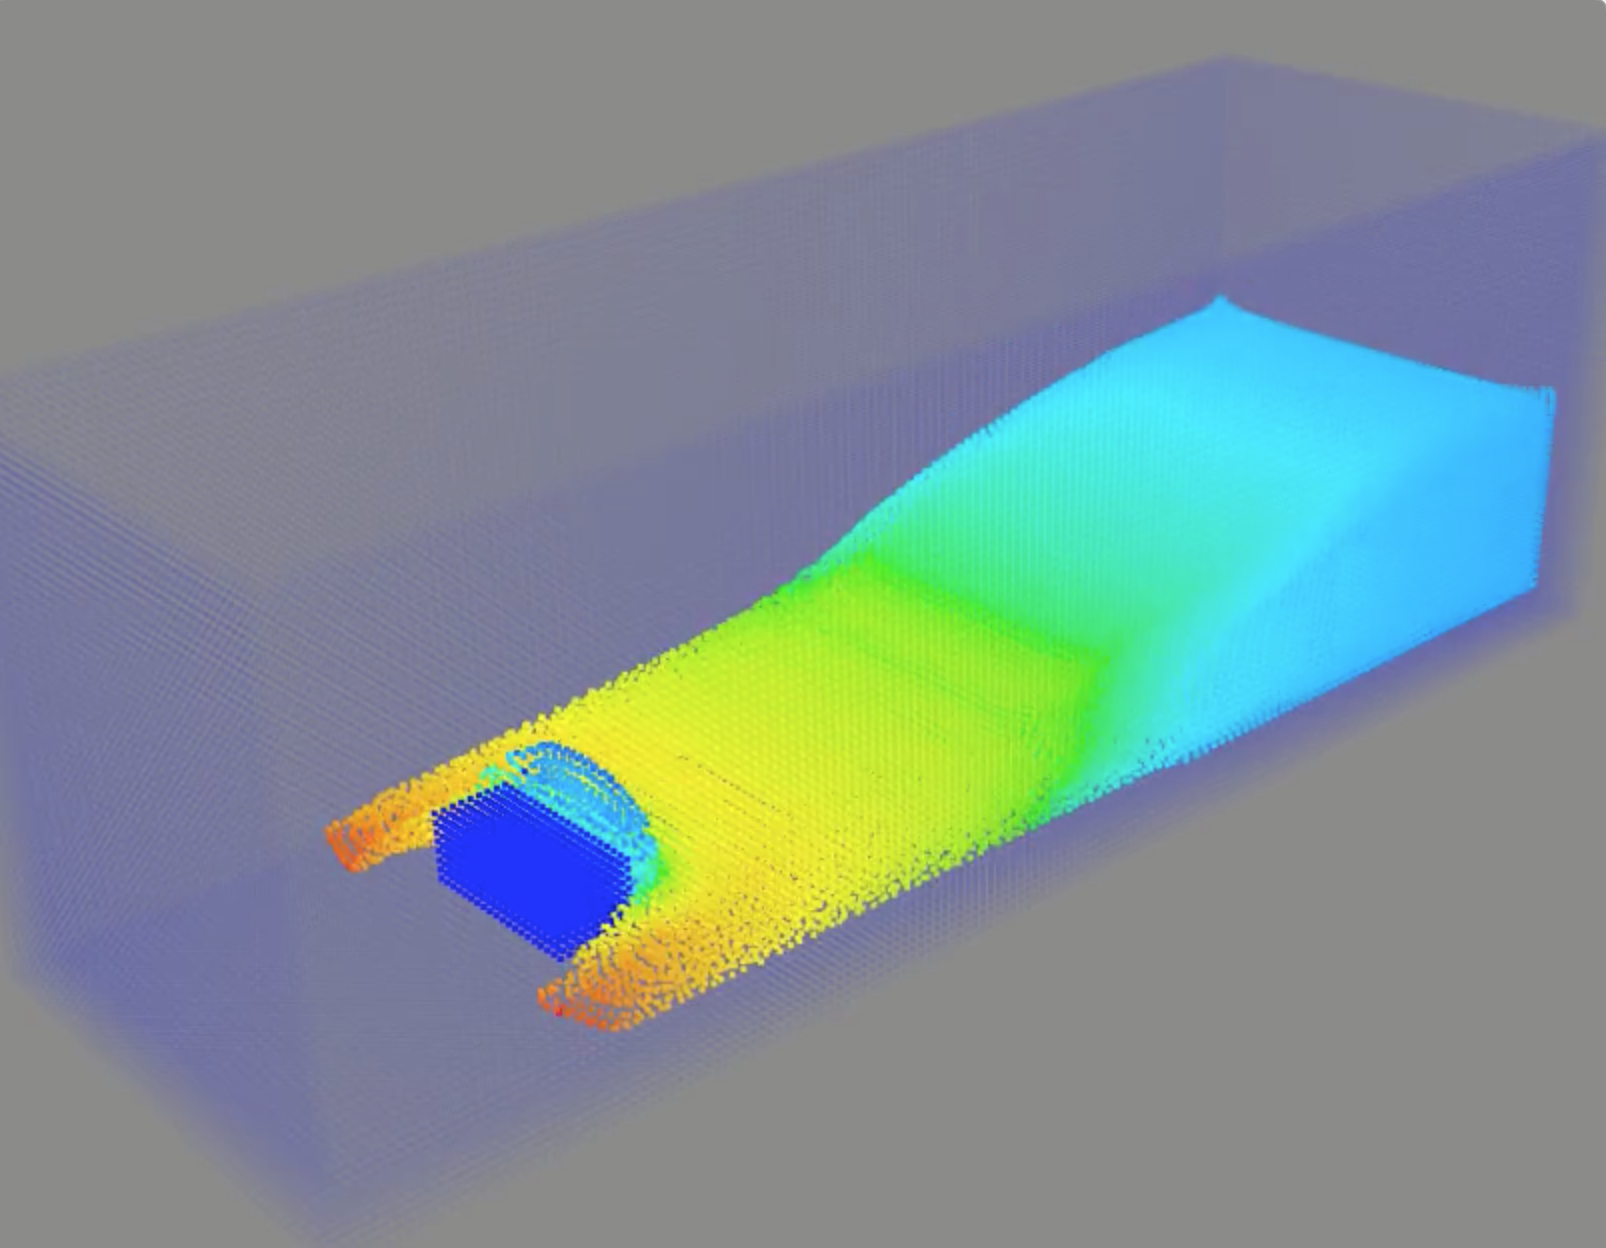
\includegraphics[height=1.75in]{data/intro/dam_break_poster}
  \end{center}
\end{frame}

\begin{frame}[plain]
  \frametitle{Requirement: UI}

  \begin{center}
    \pgfimage[height=3.25in]{data/intro/wxpy_demo}

  \end{center}

\end{frame}

\begin{frame}[plain, fragile]
    \frametitle{Super-simple UIs}
%\footnotesize
\begin{lstlisting}
from traits.api import *
class Person(HasTraits):
    name = Str('name')
    age = Range(0.0, 200.0)
    sex = Enum('male', 'female')

p = Person(name='Ram')
p.configure_traits()
\end{lstlisting}
\hrule
\pgfimage[width=0.5\textwidth, interpolate=true]{data/intro/traits_ui_wx}
\pgfimage[width=0.5\textwidth, interpolate=true]{data/intro/traits_ui_qt}
\begin{center}WxPython/Qt
\end{center}
\end{frame}



\BackgroundPicture{data/intro/django_page}
\begin{frame}[plain]
\end{frame}
\BackgroundPicture{data/intro/blank}

\begin{frame}[plain,fragile]
    \frametitle{Easy to read and still compact?}
    \footnotesize
    \begin{lstlisting}
def qsort(L):
    """Quick sort for given sequence, `L`."""
    if not L: return L # exit recursion if input is empty
    pivot, rest = L[0], L[1:]
    less_than = [ lt for lt in rest if lt < pivot ]
    greater_eq = [ ge for ge in rest if ge >= pivot ]
    return qsort(less_than) + [pivot] + qsort(greater_eq)

    \end{lstlisting}
\end{frame}

\begin{frame}[plain]
    \Huge
    \begin{center}

    \structure{Python users?}
    \end{center}
\end{frame}

\BackgroundPictureWidth{data/intro/python-orgs}
\begin{frame}[plain]
\end{frame}
\BackgroundPicture{data/intro/blank}

\begin{frame}[plain]
  \emphbar{\Large  \hfill Diverse needs, one language \hfill }
  \emphbar{\Large  \hfill Python! \hfill}
    \begin{center}
        %\structure{Python!}
    \pgfimage[height=2in]{data/intro/python_only_logo}

    \url{www.python.org}
    \end{center}

\end{frame}


\end{document}
